% Options for packages loaded elsewhere
\PassOptionsToPackage{unicode}{hyperref}
\PassOptionsToPackage{hyphens}{url}
%
\documentclass[
  man,floatsintext]{apa6}
\usepackage{amsmath,amssymb}
\usepackage{lmodern}
\usepackage{iftex}
\ifPDFTeX
  \usepackage[T1]{fontenc}
  \usepackage[utf8]{inputenc}
  \usepackage{textcomp} % provide euro and other symbols
\else % if luatex or xetex
  \usepackage{unicode-math}
  \defaultfontfeatures{Scale=MatchLowercase}
  \defaultfontfeatures[\rmfamily]{Ligatures=TeX,Scale=1}
\fi
% Use upquote if available, for straight quotes in verbatim environments
\IfFileExists{upquote.sty}{\usepackage{upquote}}{}
\IfFileExists{microtype.sty}{% use microtype if available
  \usepackage[]{microtype}
  \UseMicrotypeSet[protrusion]{basicmath} % disable protrusion for tt fonts
}{}
\makeatletter
\@ifundefined{KOMAClassName}{% if non-KOMA class
  \IfFileExists{parskip.sty}{%
    \usepackage{parskip}
  }{% else
    \setlength{\parindent}{0pt}
    \setlength{\parskip}{6pt plus 2pt minus 1pt}}
}{% if KOMA class
  \KOMAoptions{parskip=half}}
\makeatother
\usepackage{xcolor}
\IfFileExists{xurl.sty}{\usepackage{xurl}}{} % add URL line breaks if available
\IfFileExists{bookmark.sty}{\usepackage{bookmark}}{\usepackage{hyperref}}
\hypersetup{
  pdftitle={EXAMPLE PSYC 2530 HONORS PROJECT: Testing the type-token individuation theory of repetition blindness},
  pdfauthor={Matthew J. C. Crump1},
  pdflang={en-EN},
  pdfkeywords={Repetition blindness, type-token},
  hidelinks,
  pdfcreator={LaTeX via pandoc}}
\urlstyle{same} % disable monospaced font for URLs
\usepackage{graphicx}
\makeatletter
\def\maxwidth{\ifdim\Gin@nat@width>\linewidth\linewidth\else\Gin@nat@width\fi}
\def\maxheight{\ifdim\Gin@nat@height>\textheight\textheight\else\Gin@nat@height\fi}
\makeatother
% Scale images if necessary, so that they will not overflow the page
% margins by default, and it is still possible to overwrite the defaults
% using explicit options in \includegraphics[width, height, ...]{}
\setkeys{Gin}{width=\maxwidth,height=\maxheight,keepaspectratio}
% Set default figure placement to htbp
\makeatletter
\def\fps@figure{htbp}
\makeatother
\setlength{\emergencystretch}{3em} % prevent overfull lines
\providecommand{\tightlist}{%
  \setlength{\itemsep}{0pt}\setlength{\parskip}{0pt}}
\setcounter{secnumdepth}{-\maxdimen} % remove section numbering
% Make \paragraph and \subparagraph free-standing
\ifx\paragraph\undefined\else
  \let\oldparagraph\paragraph
  \renewcommand{\paragraph}[1]{\oldparagraph{#1}\mbox{}}
\fi
\ifx\subparagraph\undefined\else
  \let\oldsubparagraph\subparagraph
  \renewcommand{\subparagraph}[1]{\oldsubparagraph{#1}\mbox{}}
\fi
\newlength{\cslhangindent}
\setlength{\cslhangindent}{1.5em}
\newlength{\csllabelwidth}
\setlength{\csllabelwidth}{3em}
\newlength{\cslentryspacingunit} % times entry-spacing
\setlength{\cslentryspacingunit}{\parskip}
\newenvironment{CSLReferences}[2] % #1 hanging-ident, #2 entry spacing
 {% don't indent paragraphs
  \setlength{\parindent}{0pt}
  % turn on hanging indent if param 1 is 1
  \ifodd #1
  \let\oldpar\par
  \def\par{\hangindent=\cslhangindent\oldpar}
  \fi
  % set entry spacing
  \setlength{\parskip}{#2\cslentryspacingunit}
 }%
 {}
\usepackage{calc}
\newcommand{\CSLBlock}[1]{#1\hfill\break}
\newcommand{\CSLLeftMargin}[1]{\parbox[t]{\csllabelwidth}{#1}}
\newcommand{\CSLRightInline}[1]{\parbox[t]{\linewidth - \csllabelwidth}{#1}\break}
\newcommand{\CSLIndent}[1]{\hspace{\cslhangindent}#1}
\ifLuaTeX
\usepackage[bidi=basic]{babel}
\else
\usepackage[bidi=default]{babel}
\fi
\babelprovide[main,import]{english}
% get rid of language-specific shorthands (see #6817):
\let\LanguageShortHands\languageshorthands
\def\languageshorthands#1{}
% Manuscript styling
\usepackage{upgreek}
\captionsetup{font=singlespacing,justification=justified}

% Table formatting
\usepackage{longtable}
\usepackage{lscape}
% \usepackage[counterclockwise]{rotating}   % Landscape page setup for large tables
\usepackage{multirow}		% Table styling
\usepackage{tabularx}		% Control Column width
\usepackage[flushleft]{threeparttable}	% Allows for three part tables with a specified notes section
\usepackage{threeparttablex}            % Lets threeparttable work with longtable

% Create new environments so endfloat can handle them
% \newenvironment{ltable}
%   {\begin{landscape}\begin{center}\begin{threeparttable}}
%   {\end{threeparttable}\end{center}\end{landscape}}
\newenvironment{lltable}{\begin{landscape}\begin{center}\begin{ThreePartTable}}{\end{ThreePartTable}\end{center}\end{landscape}}

% Enables adjusting longtable caption width to table width
% Solution found at http://golatex.de/longtable-mit-caption-so-breit-wie-die-tabelle-t15767.html
\makeatletter
\newcommand\LastLTentrywidth{1em}
\newlength\longtablewidth
\setlength{\longtablewidth}{1in}
\newcommand{\getlongtablewidth}{\begingroup \ifcsname LT@\roman{LT@tables}\endcsname \global\longtablewidth=0pt \renewcommand{\LT@entry}[2]{\global\advance\longtablewidth by ##2\relax\gdef\LastLTentrywidth{##2}}\@nameuse{LT@\roman{LT@tables}} \fi \endgroup}

% \setlength{\parindent}{0.5in}
% \setlength{\parskip}{0pt plus 0pt minus 0pt}

% Overwrite redefinition of paragraph and subparagraph by the default LaTeX template
% See https://github.com/crsh/papaja/issues/292
\makeatletter
\renewcommand{\paragraph}{\@startsection{paragraph}{4}{\parindent}%
  {0\baselineskip \@plus 0.2ex \@minus 0.2ex}%
  {-1em}%
  {\normalfont\normalsize\bfseries\itshape\typesectitle}}

\renewcommand{\subparagraph}[1]{\@startsection{subparagraph}{5}{1em}%
  {0\baselineskip \@plus 0.2ex \@minus 0.2ex}%
  {-\z@\relax}%
  {\normalfont\normalsize\itshape\hspace{\parindent}{#1}\textit{\addperi}}{\relax}}
\makeatother

% \usepackage{etoolbox}
\makeatletter
\patchcmd{\HyOrg@maketitle}
  {\section{\normalfont\normalsize\abstractname}}
  {\section*{\normalfont\normalsize\abstractname}}
  {}{\typeout{Failed to patch abstract.}}
\patchcmd{\HyOrg@maketitle}
  {\section{\protect\normalfont{\@title}}}
  {\section*{\protect\normalfont{\@title}}}
  {}{\typeout{Failed to patch title.}}
\makeatother
\keywords{Repetition blindness, type-token\newline\indent Word count: 2331}
\usepackage{csquotes}
\ifLuaTeX
  \usepackage{selnolig}  % disable illegal ligatures
\fi

\title{EXAMPLE PSYC 2530 HONORS PROJECT: Testing the type-token individuation theory of repetition blindness}
\author{Matthew J. C. Crump\textsuperscript{1}}
\date{}


\shorttitle{Repetition blindness}

\authornote{

This is an EXAMPLE experiment proposal submitted as an honors project for PSYC 2530: Introductory Cognitive Psychology, Spring 2022.

Correspondence concerning this article should be addressed to Matthew J. C. Crump, . E-mail: \href{mailto:mcrump@brooklyn.cuny.edu}{\nolinkurl{mcrump@brooklyn.cuny.edu}}

}

\affiliation{\vspace{0.5cm}\textsuperscript{1} Brooklyn College of the City University of New York}

\abstract{
Repetition blindness is the finding that people can have difficulty recalling repeated items (Kanwisher, 1987). The purpose of this experiment proposal is to test predictions of the type-token individuation account of the repetition blindness effect. The experiment proposes to manipulate whether people see repeated words or repeated nonsense strings of letters. Predictions for performance in each condition are considered in relation to the type-token individuation account.
}



\begin{document}
\maketitle

How do people distinguish between multiple instances of the same thing? The literature on repetition blindness shows people can be poor at recognizing repetitions when they are presented quickly. This paper proposes an experiment to test a theoretical explanation of repetition blindness known as the type-token individuation account. \footnote{This is an example paper showing expectations for the honors project assignment in PSYC 2530. This paper uses repetition blindness as an example of a cognitive phenomena. The purpose of the honors project is to propose an experiment to test a theoretical explanation of a cognitive phenomena. This example proposal describes a test of Kanwisher's (1987) type-token individuation account. Importantly, the repetition blindness is fairly large, and many papers have been published since 1987 that used experiments to test the same hypothesis (and others). Some of the experiment ideas developed here have already been conducted by other people. Although proposing a novel experiment would be great for this honors project it is not required. The more important aspect is to engage in the process of creative scientific thinking and generate an experiment idea capable of testing predictions of a theoretical explanation. If it turns out your experiment proposal has already been conducted, that is OK.}

First, I will further describe the repetition blindness phenomena with examples. Second, I will describe how the type-token individuation theory explains repetition blindness. Third, I will develop testable predictions from the theory. Fourth, I will propose an experiment to test the predictions. Finally, I will describe possible results from the experiment that would support inferences about the type-token individuation account of repetition blindness.

\hypertarget{repetition-blindness}{%
\section{Repetition blindness}\label{repetition-blindness}}

If you have ever re-read your own writing and noticed that you accidentally typed or wrote the same word twice in a row you may have experienced repetition blindness. In this case, a typist writes a sentence and accidentally doubles a word, but fails to notice and correct the doubled word until later re-reading the text.

\begin{figure}

{\centering 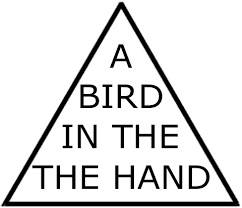
\includegraphics[width=2in]{bird_in_the_the_hand} 

}

\caption{The sentence in contains a doubled word, *the*, which is printed twice. People commonly report failing to see the second instance of *the*, producing a feeling of repetition blindness.}\label{fig:bird}
\end{figure}

Another compelling example is depicted in the figure. At first glance, many people read the sentence as ``A bird in the hand'', which is incorrect. The sentence contains \emph{the} twice, and is written as ``A bird in the \textbf{the} hand''. The experience of reading the sentence and missing the second instance of the word \emph{the} could be a form of repetition blindness.

Kanwisher (1987) reported a method to demonstrate the phenomena of repetition blindness under controlled laboratory conditions. Since 1987 many other researchers have produced reliable laboratory demonstrations of repetition blindness (for a review see, Arnell \& Shapiro, 2011). This proposal focuses on Kanwisher's original procedure, results, and interpretation.

In her first experiment, Kanwisher presented participants with a stream of seven rapidly presented words on a computer screen. For example, a participant might see the words ``TIGER, truck, APPLE, TRUCK, wagon, TRAIN, guitar'' flash very quickly in the center of the screen. Words were presented at rates between 117 ms and 250 ms each. Participants were instructed to view the stream of words, then name the repeated word and give a confidence rating. For example, in the above list the word ``truck'' appeared twice, once in lowercase and once in uppercase. Participants completed many trials, each involving a stream of words where they attempted to name the repeated word. Across trials, the location of the repeated word in the sequence was manipulated between lag 1 (one word in between the repeated words) to lag 6 (six words in between).

The results showed that accuracy for naming the repeated word decreased as a function of presentation rate and lag. Specifically, accuracy was worse as the words in the stream were presented at faster rates. And, accuracy decreased as the lag decreased. Taken together, when the repeated words were presented quickly and close together in time, participants were very poor at naming the repeated word. This effect was termed repetition blindness (RB).

\hypertarget{explaining-rb-type-token-individuation-theory}{%
\section{Explaining RB: Type-token individuation theory}\label{explaining-rb-type-token-individuation-theory}}

Kanwisher (1987) proposed several possible explanations of repetition blindness and used experiments to rule out potential explanations. For example, the recognition failure hypothesis was that people failed to detect the repeated word because all of the words were hard to recognize due to the fast presentation speeds. The rapid forgetting hypothesis was that people could have encoded the first presentation of the word, but quickly forgotten it by the time the second word was presented. The multiple comparisons hypothesis suggests that people were deliberately comparing each word in the stream with each other to check for repetitions; and, the process of deliberating comparing two words could be time-consuming and cognitively demanding causing people to miss repetitions that are presented too quickly.

These potential hypotheses were ruled out by additional experiments. For example, in her second experiment Kanwisher presented rapid streams of words in sentences and had participants recall the whole sentence. Some sentences contained repeated words like, ``When she spilled the \emph{ink} there was \emph{ink} all over.'' Other sentences served as controls, like ``When she spilled the \emph{liquid} there was \emph{ink} all over.'' Some sentences omitted the first repetition of the word, and produced ungrammatical sentences like, ``When she spilled the \emph{ink} there was all over.'' In this experiment participants showed very good recall of most words in the sentences, which ruled out the recognition failure and rapid forgetting hypotheses. However, participants were still very poor at recalling the second instance of the repeated word.

Repetition blindness occurred even when words were presented in a sentence context (just like the bird in the hand example at the beginning). An implication of this result was that participants were not deliberately comparing each word for repetitions, they were probably just trying to read the sentence. So, the result does not support the multiple-comparisons hypothesis (i.e., repetition blindness was observed even when people were just reading a sentence and not actively trying to compare words for repetitions).

Kanwisher (1987) proposed a type-token individuation hypothesis to explain her repetition blindness effects. According to this hypothesis word stimuli are assumed to activate ``type'' nodes, possibly located in an abstract semantic neural network. For example, people can see a word printed in different formats, and extract the same semantic meaning from each version of the word (e.g., ``tiger'', ``TIGER'', or \textbf{tiger}, are printed differently but have the same semantic meaning). According to the ``type'' node concept, all of the different formats of the word would activate the same type node (e.g., any version of tiger will activate the type node for \emph{tiger}). Kanwisher further proposed a ``token-individuation'' process that is responsible for distinguishing between different instances (tokens) of the same item. For example, if you read ``tiger, tiger, tiger'' at a normal speed, then you would have activated the type node for tiger, and you would have token-individuated each of the three instances of tiger. Remember, Kanwisher presented words at very fast rates, and she hypothesized that once a type node is activated the process of token individuation may be unavailable for a short duration. For example, if a first instance of ``tiger'' is presented it would activate the type node, and for a very short duration afterwards if another instance of ``tiger'' was presented, the token individuation process would fail to distinguish the second version from the first. To recap, Kanwisher suggests repetition blindness is caused by a hypothesized type-token individuation process that fails to work properly at high presentation rates.

\hypertarget{developing-testable-predictions}{%
\subsubsection{Developing testable predictions}\label{developing-testable-predictions}}

The type-token individuation account of repetition blindness implies the existence of type node representations, token representations, and a process for individuating token representations from each other and from type node representations. However, the theory as developed by Kanwisher (1987) does not fully describe many details of the above representations and processes. For example, the processing operations that allow one token to be represented as a distinct item from a repetition are not clearly specified. Similarly, although the existence of type nodes are proposed, the processes responsible for creating type nodes, or activating them by an incoming token are not clear. Because the processing assumptions of the theory are not totally clear, this proposal will develop testable predictions that apply to possible interpretations of the theory.

I will focus on the concept of the type node, which is critical to the explanation of repetition blindness. In the account, when a type node is activated by the first instance of the word, it causes a brief failure of token-individuation for repeated instances of the type. Words are assumed to have pre-existing type nodes. An outstanding question is whether repetition blindness can be observed for other kinds of stimuli besides words.

The theory appears to make one clear prediction. First, repetition blindness should occur in general for rapidly presented stimuli that have pre-existing type node representations. For example, people could have pre-existing type nodes for individual letters and numbers. This implies that people would show repetition blindness for repeated letters and numbers in a rapid stream.

What about stimuli that do not have pre-existing type node representations? One possibility is that repetition blindness will not occur for novel stimuli because they do not have pre-existing type nodes (which are presumed to be critical in causing repetition blindness). The theory is not clear on how type node representations are created. One possibility is that new stimuli (e.g., like a squiggly line that you never saw before) trigger the creation of a new type node for the novel stimulus. Assuming that creating a new type node takes time and cognitive resources could imply larger repetition blindness effects may be observed for novel stimuli.

\hypertarget{proposed-experiment}{%
\section{Proposed Experiment}\label{proposed-experiment}}

I am proposing an experiment to test the hypothetical role of type nodes in producing repetition blindness for non-word stimuli. The previous studies discussed showed repetition blindness for repeated word stimuli, which are presumed to have pre-existing type nodes.

My experiment will use the same general method as Kanwisher (1987), but the major manipulation will be to change the kinds of stimuli shown in the rapid stream of items.

I will include the following classes of stimuli. In the word condition, I will present sequences of 7 words. In the letter condition, I will present sequences of 7 letters. In the number condition, I will present sequences of Arabic digits. In the squiggle condition, I will present sequences of unfamiliar line squiggle drawings. In the unfamiliar alphabet condition, I will present sequences of characters from a fake alien language that no one has ever seen before (that will be invented for this experiment).

Every sequence of items will either contain one repeated item at different lags; or will not contain a repeated item. The sequences will be presented at 100ms per item. Participants will be shown each sequence, and then asked to judge whether the stream contained a repeated item or not.

\hypertarget{predicted-results}{%
\section{Predicted Results}\label{predicted-results}}

If people are susceptible to repetition blindness, then accuracy for judging whether the sequence contained a repeated item should be worse for sequences containing a repeated item compared to sequences not containing a repeated item.

If type nodes are required for repetition blindness, then I predict that repetition blindness will be observed for the word, letter, and digit streams. Word, letter, and digit stimuli should have pre-existing type nodes. According to the type-token individuation theory, these stimuli will suffer from repetition blindness when they are repeated in rapidly presented lists. Specifically, participants should have low accuracy in judging whether or not a sequence of words, letters, or digits contains a repeated item.

Similarly, if type nodes are required for repetition blindness, then I predict that repetition blindness may not be observed for sequences of squiggles and unfamiliar alphabet stimuli. These stimuli are novel and should not have pre-existing type nodes, so it is not clear that repetition blindness will be observed for these items. Thus, it is possible that accuracy for judging whether a stream contains a repeated item will be much higher for these items, compared to familiar stimuli with type nodes.

Alternatively, it is possible that repetition blindness will be observed for the novel stimuli. The type-token individuation theory could be extended to account for this finding. For example, it is possible that new unfamiliar items trigger the creation of a new type. The process of creating a new type node might require even more cognitive resources than usual, and may cause the token-individuation process to fail for any repetitions of the novel item that appear rapidly after the first presentation. On this view, it is possible that repetition blindness will be even larger for novel stimuli that require type nodes to be created when they are first presented, compared to familiar stimuli that already have pre-existing type nodes.

\hypertarget{discussion}{%
\section{Discussion}\label{discussion}}

The proposed experiment is aimed at testing the type-token individuation account of repetition blindness. The results of the experiment could corroborate some predictions of the theory. For example, if repetition blindness occurs for familiar stimuli (words, letters, numbers) that are assumed to have pre-existing type nodes, then the prediction that repetition blindness depends on type nodes would be corroborated.

It is possible that repetition blindness will not occur for letter and number stimuli even though they should have pre-existing type nodes. The type-token individuation account may have to be modified to explain this kind of result.

It is less clear whether the results of the proposed experiment can falsify the type-token individuation account. The account does not make strong predictions about whether repetition blindness should occur for novel stimuli that do not have pre-existing type nodes. Finding a repetition blindness effect (or not finding one) for novel stimuli would nevertheless be theoretically informative. On the one hand, finding a repetition blindness effect could mean that type nodes are not necessary for the effect. This interpretation would suggest the need for different account of repetition blindness. On the other hand, as discussed earlier, finding a repetition blindness effect could be interpreted as new evidence for a type node creation process. Additional experiments and theory development are necessary to explain and evaluate accounts of repetition blindness.

\newpage

\hypertarget{references}{%
\section{References}\label{references}}

\begingroup
\setlength{\parindent}{-0.5in}
\setlength{\leftskip}{0.5in}

\hypertarget{refs}{}
\begin{CSLReferences}{1}{0}
\leavevmode\vadjust pre{\hypertarget{ref-arnell2011attentional}{}}%
Arnell, K. M., \& Shapiro, K. L. (2011). Attentional blink and repetition blindness. \emph{Wiley Interdisciplinary Reviews: Cognitive Science}, \emph{2}(3), 336--344.

\leavevmode\vadjust pre{\hypertarget{ref-kanwisher1987repetition}{}}%
Kanwisher, N. G. (1987). Repetition blindness: Type recognition without token individuation. \emph{Cognition}, \emph{27}(2), 117--143.

\end{CSLReferences}

\endgroup


\end{document}
